	
%% bare_conf.tex
%% V1.3
%% 2007/01/11
%% by Michael Shell
%% See:
%% http://www.michaelshell.org/
%% for current contact information.
%%
%% This is a skeleton file demonstrating the use of IEEEtran.cls
%% (requires IEEEtran.cls version 1.7 or later) with an IEEE conference paper.
%%
%% Support sites:
%% http://www.michaelshell.org/tex/ieeetran/
%% http://www.ctan.org/tex-archive/macros/latex/contrib/IEEEtran/
%% and
%% http://www.ieee.org/

%%*************************************************************************
%% Legal Notice:
%% This code is offered as-is without any warranty either expressed or
%% implied; without even the implied warranty of MERCHANTABILITY or
%% FITNESS FOR A PARTICULAR PURPOSE! 
%% User assumes all risk.
%% In no event shall IEEE or any contributor to this code be liable for
%% any damages or losses, including, but not limited to, incidental,
%% consequential, or any other damages, resulting from the use or misuse
%% of any information contained here.
%%
%% All comments are the opinions of their respective authors and are not
%% necessarily endorsed by the IEEE.
%%
%% This work is distributed under the LaTeX Project Public License (LPPL)
%% ( http://www.latex-project.org/ ) version 1.3, and may be freely used,
%% distributed and modified. A copy of the LPPL, version 1.3, is included
%% in the base LaTeX documentation of all distributions of LaTeX released
%% 2003/12/01 or later.
%% Retain all contribution notices and credits.
%% ** Modified files should be clearly indicated as such, including  **
%% ** renaming them and changing author support contact information. **
%%
%% File list of work: IEEEtran.cls, IEEEtran_HOWTO.pdf, bare_adv.tex,
%%                    bare_conf.tex, bare_jrnl.tex, bare_jrnl_compsoc.tex
%%*************************************************************************

% *** Authors should verify (and, if needed, correct) their LaTeX system  ***
% *** with the testflow diagnostic prior to trusting their LaTeX platform ***
% *** with production work. IEEE's font choices can trigger bugs that do  ***
% *** not appear when using other class files.                            ***
% The testflow support page is at:
% http://www.michaelshell.org/tex/testflow/



% Note that the a4paper option is mainly intended so that authors in
% countries using A4 can easily print to A4 and see how their papers will
% look in print - the typesetting of the document will not typically be
% affected with changes in paper size (but the bottom and side margins will).
% Use the testflow package mentioned above to verify correct handling of
% both paper sizes by the user's LaTeX system.
%
% Also note that the "draftcls" or "draftclsnofoot", not "draft", option
% should be used if it is desired that the figures are to be displayed in
% draft mode.
%
\documentclass[conference]{IEEEtran}
% Add the compsoc option for Computer Society conferences.
%
% If IEEEtran.cls has not been installed into the LaTeX system files,
% manually specify the path to it like:
% \documentclass[conference]{../sty/IEEEtran}





% Some very useful LaTeX packages include:
% (uncomment the ones you want to load)


% *** MISC UTILITY PACKAGES ***
%
%\usepackage{ifpdf}
% Heiko Oberdiek's ifpdf.sty is very useful if you need conditional
% compilation based on whether the output is pdf or dvi.
% usage:
% \ifpdf
%   % pdf code
% \else
%   % dvi code
% \fi
% The latest version of ifpdf.sty can be obtained from:
% http://www.ctan.org/tex-archive/macros/latex/contrib/oberdiek/
% Also, note that IEEEtran.cls V1.7 and later provides a builtin
% \ifCLASSINFOpdf conditional that works the same way.
% When switching from latex to pdflatex and vice-versa, the compiler may
% have to be run twice to clear warning/error messages.






% *** CITATION PACKAGES ***
%
%\usepackage{cite}
% cite.sty was written by Donald Arseneau
% V1.6 and later of IEEEtran pre-defines the format of the cite.sty package
% \cite{} output to follow that of IEEE. Loading the cite package will
% result in citation numbers being automatically sorted and properly
% "compressed/ranged". e.g., [1], [9], [2], [7], [5], [6] without using
% cite.sty will become [1], [2], [5]--[7], [9] using cite.sty. cite.sty's
% \cite will automatically add leading space, if needed. Use cite.sty's
% noadjust option (cite.sty V3.8 and later) if you want to turn this off.
% cite.sty is already installed on most LaTeX systems. Be sure and use
% version 4.0 (2003-05-27) and later if using hyperref.sty. cite.sty does
% not currently provide for hyperlinked citations.
% The latest version can be obtained at:
% http://www.ctan.org/tex-archive/macros/latex/contrib/cite/
% The documentation is contained in the cite.sty file itself.






% *** GRAPHICS RELATED PACKAGES ***
%
\ifCLASSINFOpdf
  \usepackage[pdftex]{graphicx}
  % declare the path(s) where your graphic files are
  % \graphicspath{{../pdf/}{../jpeg/}}
  % and their extensions so you won't have to specify these with
  % every instance of \includegraphics
  % \DeclareGraphicsExtensions{.pdf,.jpeg,.png}
\else
  % or other class option (dvipsone, dvipdf, if not using dvips). graphicx
  % will default to the driver specified in the system graphics.cfg if no
  % driver is specified.
  % \usepackage[dvips]{graphicx}
  % declare the path(s) where your graphic files are
  % \graphicspath{{../eps/}}
  % and their extensions so you won't have to specify these with
  % every instance of \includegraphics
  % \DeclareGraphicsExtensions{.eps}
\fi
% graphicx was written by David Carlisle and Sebastian Rahtz. It is
% required if you want graphics, photos, etc. graphicx.sty is already
% installed on most LaTeX systems. The latest version and documentation can
% be obtained at: 
% http://www.ctan.org/tex-archive/macros/latex/required/graphics/
% Another good source of documentation is "Using Imported Graphics in
% LaTeX2e" by Keith Reckdahl which can be found as epslatex.ps or
% epslatex.pdf at: http://www.ctan.org/tex-archive/info/
%
% latex, and pdflatex in dvi mode, support graphics in encapsulated
% postscript (.eps) format. pdflatex in pdf mode supports graphics
% in .pdf, .jpeg, .png and .mps (metapost) formats. Users should ensure
% that all non-photo figures use a vector format (.eps, .pdf, .mps) and
% not a bitmapped formats (.jpeg, .png). IEEE frowns on bitmapped formats
% which can result in "jaggedy"/blurry rendering of lines and letters as
% well as large increases in file sizes.
%
% You can find documentation about the pdfTeX application at:
% http://www.tug.org/applications/pdftex





% *** MATH PACKAGES ***
%
\usepackage[cmex10]{amsmath}
% A popular package from the American Mathematical Society that provides
% many useful and powerful commands for dealing with mathematics. If using
% it, be sure to load this package with the cmex10 option to ensure that
% only type 1 fonts will utilized at all point sizes. Without this option,
% it is possible that some math symbols, particularly those within
% footnotes, will be rendered in bitmap form which will result in a
% document that can not be IEEE Xplore compliant!
%
% Also, note that the amsmath package sets \interdisplaylinepenalty to 10000
% thus preventing page breaks from occurring within multiline equations. Use:
%\interdisplaylinepenalty=2500
% after loading amsmath to restore such page breaks as IEEEtran.cls normally
% does. amsmath.sty is already installed on most LaTeX systems. The latest
% version and documentation can be obtained at:
% http://www.ctan.org/tex-archive/macros/latex/required/amslatex/math/





% *** SPECIALIZED LIST PACKAGES ***
%
%\usepackage{algorithmic}
% algorithmic.sty was written by Peter Williams and Rogerio Brito.
% This package provides an algorithmic environment fo describing algorithms.
% You can use the algorithmic environment in-text or within a figure
% environment to provide for a floating algorithm. Do NOT use the algorithm
% floating environment provided by algorithm.sty (by the same authors) or
% algorithm2e.sty (by Christophe Fiorio) as IEEE does not use dedicated
% algorithm float types and packages that provide these will not provide
% correct IEEE style captions. The latest version and documentation of
% algorithmic.sty can be obtained at:
% http://www.ctan.org/tex-archive/macros/latex/contrib/algorithms/
% There is also a support site at:
% http://algorithms.berlios.de/index.html
% Also of interest may be the (relatively newer and more customizable)
% algorithmicx.sty package by Szasz Janos:
% http://www.ctan.org/tex-archive/macros/latex/contrib/algorithmicx/




% *** ALIGNMENT PACKAGES ***
%
%\usepackage{array}
% Frank Mittelbach's and David Carlisle's array.sty patches and improves
% the standard LaTeX2e array and tabular environments to provide better
% appearance and additional user controls. As the default LaTeX2e table
% generation code is lacking to the point of almost being broken with
% respect to the quality of the end results, all users are strongly
% advised to use an enhanced (at the very least that provided by array.sty)
% set of table tools. array.sty is already installed on most systems. The
% latest version and documentation can be obtained at:
% http://www.ctan.org/tex-archive/macros/latex/required/tools/


%\usepackage{mdwmath}
%\usepackage{mdwtab}
% Also highly recommended is Mark Wooding's extremely powerful MDW tools,
% especially mdwmath.sty and mdwtab.sty which are used to format equations
% and tables, respectively. The MDWtools set is already installed on most
% LaTeX systems. The lastest version and documentation is available at:
% http://www.ctan.org/tex-archive/macros/latex/contrib/mdwtools/


% IEEEtran contains the IEEEeqnarray family of commands that can be used to
% generate multiline equations as well as matrices, tables, etc., of high
% quality.


%\usepackage{eqparbox}
% Also of notable interest is Scott Pakin's eqparbox package for creating
% (automatically sized) equal width boxes - aka "natural width parboxes".
% Available at:
% http://www.ctan.org/tex-archive/macros/latex/contrib/eqparbox/





% *** SUBFIGURE PACKAGES ***
%\usepackage[tight,footnotesize]{subfigure}
% subfigure.sty was written by Steven Douglas Cochran. This package makes it
% easy to put subfigures in your figures. e.g., "Figure 1a and 1b". For IEEE
% work, it is a good idea to load it with the tight package option to reduce
% the amount of white space around the subfigures. subfigure.sty is already
% installed on most LaTeX systems. The latest version and documentation can
% be obtained at:
% http://www.ctan.org/tex-archive/obsolete/macros/latex/contrib/subfigure/
% subfigure.sty has been superceeded by subfig.sty.



%\usepackage[caption=false]{caption}
%\usepackage[font=footnotesize]{subfig}
% subfig.sty, also written by Steven Douglas Cochran, is the modern
% replacement for subfigure.sty. However, subfig.sty requires and
% automatically loads Axel Sommerfeldt's caption.sty which will override
% IEEEtran.cls handling of captions and this will result in nonIEEE style
% figure/table captions. To prevent this problem, be sure and preload
% caption.sty with its "caption=false" package option. This is will preserve
% IEEEtran.cls handing of captions. Version 1.3 (2005/06/28) and later 
% (recommended due to many improvements over 1.2) of subfig.sty supports
% the caption=false option directly:
%\usepackage[caption=false,font=footnotesize]{subfig}
%
% The latest version and documentation can be obtained at:
% http://www.ctan.org/tex-archive/macros/latex/contrib/subfig/
% The latest version and documentation of caption.sty can be obtained at:
% http://www.ctan.org/tex-archive/macros/latex/contrib/caption/




% *** FLOAT PACKAGES ***
%
%\usepackage{fixltx2e}
% fixltx2e, the successor to the earlier fix2col.sty, was written by
% Frank Mittelbach and David Carlisle. This package corrects a few problems
% in the LaTeX2e kernel, the most notable of which is that in current
% LaTeX2e releases, the ordering of single and double column floats is not
% guaranteed to be preserved. Thus, an unpatched LaTeX2e can allow a
% single column figure to be placed prior to an earlier double column
% figure. The latest version and documentation can be found at:
% http://www.ctan.org/tex-archive/macros/latex/base/



%\usepackage{stfloats}
% stfloats.sty was written by Sigitas Tolusis. This package gives LaTeX2e
% the ability to do double column floats at the bottom of the page as well
% as the top. (e.g., "\begin{figure*}[!b]" is not normally possible in
% LaTeX2e). It also provides a command:
%\fnbelowfloat
% to enable the placement of footnotes below bottom floats (the standard
% LaTeX2e kernel puts them above bottom floats). This is an invasive package
% which rewrites many portions of the LaTeX2e float routines. It may not work
% with other packages that modify the LaTeX2e float routines. The latest
% version and documentation can be obtained at:
% http://www.ctan.org/tex-archive/macros/latex/contrib/sttools/
% Documentation is contained in the stfloats.sty comments as well as in the
% presfull.pdf file. Do not use the stfloats baselinefloat ability as IEEE
% does not allow \baselineskip to stretch. Authors submitting work to the
% IEEE should note that IEEE rarely uses double column equations and
% that authors should try to avoid such use. Do not be tempted to use the
% cuted.sty or midfloat.sty packages (also by Sigitas Tolusis) as IEEE does
% not format its papers in such ways.





% *** PDF, URL AND HYPERLINK PACKAGES ***
%
%\usepackage{url}
% url.sty was written by Donald Arseneau. It provides better support for
% handling and breaking URLs. url.sty is already installed on most LaTeX
% systems. The latest version can be obtained at:
% http://www.ctan.org/tex-archive/macros/latex/contrib/misc/
% Read the url.sty source comments for usage information. Basically,
% \url{my_url_here}.





% *** Do not adjust lengths that control margins, column widths, etc. ***
% *** Do not use packages that alter fonts (such as pslatex).         ***
% There should be no need to do such things with IEEEtran.cls V1.6 and later.
% (Unless specifically asked to do so by the journal or conference you plan
% to submit to, of course. )


% correct bad hyphenation here
\hyphenation{op-tical net-works semi-conduc-tor}


\begin{document}
%
% paper title
% can use linebreaks \\ within to get better formatting as desired
\title{Paraphrasing in Twitter}


% author names and affiliations
% use a multiple column layout for up to three different
% affiliations
\author{\IEEEauthorblockN{Melvin Johnson Premkumar}
\IEEEauthorblockA{Dept. of Computer Science\\
Stanford University\\
Email: melvinj@stanford.edu}
\and
\IEEEauthorblockN{Isaac Caswell}
\IEEEauthorblockA{Dept. of Computer Science\\
Stanford University\\
Email: icaswell@stanford.edu}
\and
\IEEEauthorblockN{Zane Silver}
\IEEEauthorblockA{Dept. of Electrical Engineering\\
Stanford University\\
Email: zsilver@stanford.edu}}

% conference papers do not typically use \thanks and this command
% is locked out in conference mode. If really needed, such as for
% the acknowledgment of grants, issue a \IEEEoverridecommandlockouts
% after \documentclass

% for over three affiliations, or if they all won't fit within the width
% of the page, use this alternative format:
% 
%\author{\IEEEauthorblockN{Michael Shell\IEEEauthorrefmark{1},
%Homer Simpson\IEEEauthorrefmark{2},
%James Kirk\IEEEauthorrefmark{3}, 
%Montgomery Scott\IEEEauthorrefmark{3} and
%Eldon Tyrell\IEEEauthorrefmark{4}}
%\IEEEauthorblockA{\IEEEauthorrefmark{1}School of Electrical and Computer Engineering\\
%Georgia Institute of Technology,
%Atlanta, Georgia 30332--0250\\ Email: see http://www.michaelshell.org/contact.html}
%\IEEEauthorblockA{\IEEEauthorrefmark{2}Twentieth Century Fox, Springfield, USA\\
%Email: homer@thesimpsons.com}
%\IEEEauthorblockA{\IEEEauthorrefmark{3}Starfleet Academy, San Francisco, California 96678-2391\\
%Telephone: (800) 555--1212, Fax: (888) 555--1212}
%\IEEEauthorblockA{\IEEEauthorrefmark{4}Tyrell Inc., 123 Replicant Street, Los Angeles, California 90210--4321}}




% use for special paper notices
%\IEEEspecialpapernotice{(Invited Paper)}




% make the title area
\maketitle

% IEEEtran.cls defaults to using nonbold math in the Abstract.
% This preserves the distinction between vectors and scalars. However,
% if the conference you are submitting to favors bold math in the abstract,
% then you can use LaTeX's standard command \boldmath at the very start
% of the abstract to achieve this. Many IEEE journals/conferences frown on
% math in the abstract anyway.

% no keywords


% For peer review papers, you can put extra information on the cover
% page as needed:
% \ifCLASSOPTIONpeerreview
% \begin{center} \bfseries EDICS Category: 3-BBND \end{center}
% \fi
%
% For peerreview papers, this IEEEtran command inserts a page break and
% creates the second title. It will be ignored for other modes.
\IEEEpeerreviewmaketitle



\begin{abstract}
Our project is detecting and identifying paraphrases in Twitter, as part of the SemEval challenge for 2015.   Given two sentences (tweets), we determine whether they express the same, or very similar, meaning.  The training dataset is provided by semEval and contains about 17,790 annotated sentence pairs, and comes with tokenization, part-of-speech and named entity tags. SemEval also provides two baselines against which to compare our algorithm's performance. We experimented with different word vector representations trained using different techniques. We also tried various features and performed feature selection to select the best features. We also experimented with different classifiers for the task. Our final best system obtains a precision of \textbf{0.665}, recall of \textbf{0.422}, F1 of \textbf{0.517} and an accuracy of 0.75. We worked in collaboration with  Xiao Cheng, a PhD candidate in the Computer Science Dept.\\ 
\end{abstract}

% You must have at least 2 lines in the paragraph with the drop letter
% (should never be an issue)
\section{Introduction}
\subsection{Task Review}
Given two phrases, we determine whether they express the same or very similar meaning. The input to the system is two sentences from tweets in Twitter. The system predicts whether they express the same meaning.  System performance is evaluated by SemEval primarily by the F-1 score and Accuracy against human judgements.\\


\subsection{Challenges in Paraphrasing \& Analysis of Tweets}
Paraphrase detection as a field has recently attracted interest, with the hope that solving the task might help shed light on how best to model the semantics of sentences.  The potential applications of a good framework are wide-ranging: ``For natural language engineers, the problem bears on information management systems like abstractive summarizers that must measure semantic overlap between sentences (Barzilay and Lee, 2003), question answering modules (Marsi and Krahmer, 2005) and machine translation (Callison-Burch et al., 2006)." \cite{Das}
\indent As with any task which deals with the semantics of natural language, accurately identifying related paraphrases is very difficult.  It is not enough to determine that two sentences refer to the same thing, which is already a nontrivial task; they must also refer to the same thing in the same context and relation to the other variables in the sentence.  The meaning a sentence, especially a short one such as a tweet, is also heavily dependant on the context it was written in.  With our dataset, for instance, time, place and knowledge of current events (especially sports) play a large role in understanding of a tweet. Not only is the meaning of a tweet hypersensitive to time and location, but tweets also frequently contain linguistic errors and idiosyncratic styles \cite{derczynski}. Additionally, the limit in the number of characters of a tweet constrains the ability to provide contextual meaning to the phrase. For this reason, other indicators may become more important in deciphering a tweet's meaning: time, location, slang, and so on.\\
\indent There are several ways of ameliorating some of these difficulties, including normalizing the data (e.g. correcting spelling, stemming) and improving the library of English parts-of-speech \cite{derczynski}. Additionally, it helps to understand the use of tweets and the specific characteristics of different uses. For example, using tweets for political news updates is much different than celebrity gossip or rumors \cite{OConnor}.  The data provided by semEval has already been preprocessed to a certain degree, dealing with some of these issues.  Nonetheless, the hardest part remains: dealing with the semantics.
\subsection{Paper Flow}
\noindent We will first discuss the training and testing data we used, including preprocessing of the data.   The oracle and baseline will then be detailed.  Following this we describe the underpinnings and capabilities of distributional word representations (dense word vectors), and why they make sense for this problem.  With this in place, we describe our method for comparing two tweets, and how to learn word vectors with the Skip-gram model.  Thereafter we describe three other approaches we use, namely Unfolding Recursive Autoencoders, GloVe vectors, and a classifier with features derived from word vectors and other sources.  Finally, we discuss results, give an error analysis, conclude, and suggest directions for future work.
\section{Data description and Preprocessing}
\subsection {Train and Test Data} 
Our training data (provided by SemEval) consists of 18k representative tweets semi-randomly collected from Twitter's feed, annotated by several Mechanical Turkers.  The data is balanced (appx. 35\% paraphrase, 65\% non-paraphrase), and have already been tokenized and split into sentences.  Part of speech (POS) tagging is also provided. Hashtags were removed.  The test set  consists of a further 1k data from a different time period, annotated by an expert.  In summary:

\begin{table}[h]
\begin{tabular}{lllll}
           & sentence pairs & fraction paraphrase & fraction not paraphrase &  \\
\hline
train data & 13063          & .35                 & 0.65                    &  \\
test data  & 4727           & (unreleased)                & (unreleased)                    & 
\end{tabular}
\end{table}

\subsection{Preprocessing step: normalization of the data}
Twitter datasets tend to attract slang and misspellings, arbitrary capitalization and the like.  For this reason we normalize our data first with TODO.  We have found an external library (twitter lexicon normalization) which....we will apply this to our dataset and see what the effect on our performance is.  This tool can be used with a Twitter specifc entity detector, availiable online at https://github.com/sem-io/python-twitter-spell-checking. Furthermore one could experiment with basic word stemming.  


\subsection{Additional Training Corpuses Used}
We used three different corpuses to train our word vectors:\\
\begin{itemize}
\item \textbf{googleNews}: a dataset of articles from Google News, containing about 100 billion tokens and  692K types (after removing words ocurring less than 5 times).
\item \textbf{wiki\_giga.txt}: Aka Gigaword, the English Gigaword Fifth Edition corpus (released June 17, 2011), an archive of 4.3 billion tokens from newswire text data in English that has been acquired over several years by the Linguistic Data Consortium at the University of Pennsylvania.  \cite{GloVe} \cite{Gigaword}.  Contains text from theEnglish service of the Associated Press Worldstream, the Central News Agency of Taiwan, the Los Angeles Times/Washington Post Newswire, the Washington Post/Bloomberg Newswire and the New York Times Newswire and Xinhua News Agency.
\item \textbf{wiki\_giga\_skipgram.txt}: the combination of Gigaword5 and Wikipedia2014, a Wikipedia dump.  The combined dataset has 6 billion tokens.
\item \textbf{twitterGlove}: a dataset of about 2 billion tweets, with 27 billion tokens total.

\end{itemize}

\subsection{Oracle}
The oracle for our twitter phase classifier are human identifiers. This relies on humans reading two different twitter phrases and determining whether or not they refer to the same context. The added constraints are that the phrase identification must be performed in a timely manner (under a minute per phrase pair) and without outside help (i.e. searching on the internet the meaning of a word, phrase, etc.).  To test the a performance of the oracle, we tested one of our own members on 100 tweet pairs.  His performance compared to the baseline (discussed in the next section) is summarized by the following table:

\begin{table}[h]
\begin{tabular}{lllll}
         & Precision & Recall & F1   & Accuracy \\
\hline
Oracle   & 0.60      & 0.91   & 0.74 & 0.76     \\
Baseline & 0.70      & 0.39   & 0.50 & 0.73     \\ 
\end{tabular}
\end{table}

The table highlights how difficult the task is, in that even a human evaluator does not significantly outscore the baseline.  The tweets are short and without context (e.g. \textit{``angie shud go and i want candice to win"} and \textit{``Now it s up to Candice and Amber"}), and the criteria for paraphrase can be ambiguous.  For instance, \textit{``am i the only one not getting amber alerts"} and \textit{``I need a amber alert to wake tf up in da mornings Ha"} are both about Amber Alerts, but are about different aspects of them, so it is unclear if they should count as paraphrases.

\section{Baseline Description}
As a baseline model we found the MULTIP (Multi-Instance Learning Paraphrase) model for the Twitter phrase classifier. This model was proposed by Xu et. al \cite{zane}. Their model serves as a good starting point and is the reference baseline model for our twitter classifier project. The model description below is a summary of the proposal for the MULTIP model. \\
\indent The advantage of using the MULTIP model is that it relies on sentence level relations using a feature-based classifier. Extensive research has been undertaken to improve upon the MULTIP model so that it can correctly identify two related twitter texts. This has proven to be especially difficult because of the amount of variability in the type of tweets and the prevalence of generalized naming for entities. Specifically, the paper presenting MULTIP uses the example sentences:

\begin{itemize}
\item That boy Brook Lopez with a deep 3
\item brook Lopez hit a 3 and I missed it
\end{itemize}

The above example is just to illustrate difficulty that arises when the named entities are generalized into different words. \\
\indent Firstly, the MULTIP model relies on the at-least-one-anchor assumption. The at-least-one-anchor assumption is derived from the idea that twitter messages posted around the same time and the same topic share lexical paraphrases. This intuition allows us to extend the idea further: that most related tweets, not just those posted around the same time or location, will share a lexical paraphrase. The lexical paraphrases may be the same words, or different words, that are contained in two different tweets that identity the tweets are being related. In other words, it is assumed that related tweets contain an anchor, a lexical paraphrase. In the context of CS 221, an anchor is simply a factor. \\
\indent The MULTIP model sets up a learner that observes the labels on groups of sentence-level paraphrases. This is due to the at-least-one-anchor assumption described early. This method contrasts with a learner that observes word pairs. There are now two layers in the model, since the sentence-level analysis inherently relies on the word-level analysis. This two-level hierarchy is described in explicit detail in the proposal by Xu et. al \cite{zane}. In the context of this class, the two-level model is simply a factor graph with paraphrases/sentences as the upper nodes and the word-pairs as the lower, or leaf, nodes.\\
\indent For each pair of sentences there is a binary variable $y$ that represents whether the two sentences are related. This is determined to be true ($y=1$) if there is at least one anchor found in common between the two sentences. We determine if at least one anchor exists in the set of word-pairs between the two sentences. The set of word-pairs is the set of unique word-pairs that can be formed from one word in each sentence. For each word-pair there is another binary variable $z$ which determines if those words are an anchor or not. Therefore, for $y=1$ there must be at least one $z=1$ in the set of word-pairs for the two sentences.  \\
For two sentences $s_{1}$ and $s_{2}$, y($s_{2}$,$s_{1}$) = 1 
if $z_{j}$ = 1 for at least one j. $z_{j}$ = 1 only if $w_{j}$ = ($w_{j1}$, $w_{j2}$) is an anchor, where $w_{ji}$ corresponds to a word in sentence $s_{i}$. For every sentence pair ($s_{i}$, $s_{k}$), there will be $|s_{i}|$ * $|s_{k}|$ word-pairs, where $|s_{i}|$ is the number of words in sentence $s_{i}$. \\

\indent This model suffices as a basic outline on how to solve the Twitter classifier. However, this is only our baseline as the actual model and algorithm we implement is described below.
 
 \section{Foundations: Distributional word representations}
 \noindent Our approach to solving the problem of Twitter paraphrases hinges on the application of a dense vector representation for words and phrases.  This section details the idea behind this approach, and its advantages.\\
\indent In standard applications of machine learning techniques to NLP, words have been represented by "one-hot" vectors, which are vectors whose entries are all zero except for a single 1 entry. A typical way of representing a document, for instance, is as a counts vector, or with some derivative of word counts, such as tf-idf (term frequency-inverse document frequency).  This approach yields a vector of length $|V|$ for each document, where entry $i$ corresponds to some function of the count of the $i$th word in the vocabulary.  Such a count vector can be seen as a sum of vectors for each word, where each vector is a one-hot vector with its one entry in the index corresponding to that token.  These models have been moderately successful, but suffer from some serious problems. Primarily, a one-hot word representation  doesn't offer any information about the semantics of an individual word, and ignores the local context in which the word appears. Furthermore, as a result, any reasonable measure of vector similarity between two words, with such a model, is zero.\\

\begin{figure}
	\centering
	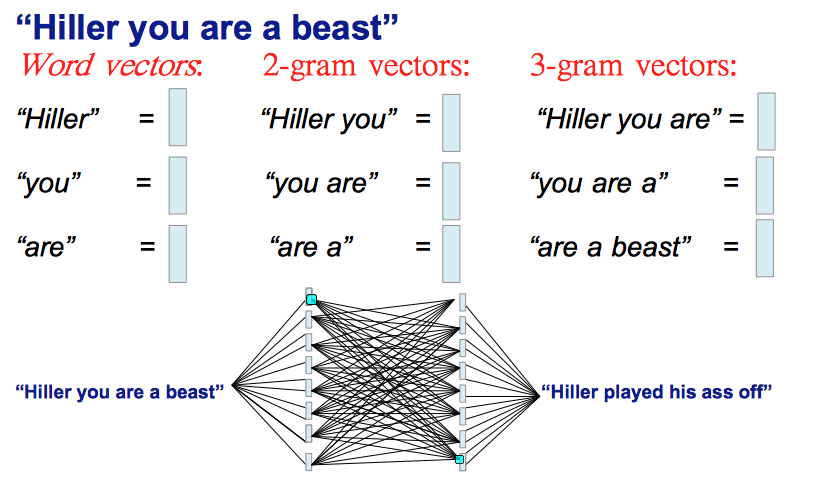
\includegraphics[scale=0.3]{tweet_cmp_cs221.png}
	\caption{Word Vectors}
	\label{fig1}
\end{figure}

\indent A one dimensional representation doesn't match what we know about words; words can be similar in certain ways, and different in others.  The words "fear" and "trembling", for instance, are similar in that they are both nouns, different in that one is emotional and the other physical; close to each other in negative valence and further from each other in commonness in standard parlance, and so on; a human could easily identify hundreds of dimensions in which they are close or far.  This is precisely the idea behind dense vector representations of words. Each word in these models is represented as a dense vector $w$, where each entry $w_k$ corresponds to some 'topic' or property of that word. (One may think $w$ as an unnormalized probability distribution over different attributes of the word.) In practice, to generate these distributions, some form of statistical clustering is performed first, usually based on which words tend to co-occur. Each dimension ('topic') is determined by the percent membership to different clusters, based on the global word co-occurrence matrix $X$ \cite{Wordvec}.\\
\indent There are a variety of advantages of this approach.  First of all, and germane to our application to the Twitter dataset, there is now a well defined and meaningful distance between words.  Distance metrics such as the cosine and Euclidean distance between two dense word vectors can give a relatively meaningful approximation of how similar these words are as a whole, which we demonstrate to be of practical use in determining similarity of tweets.\\
\indent The expressive power of word vectors is especially evident in the example of vector similarity, a metric which respects a finer-grained relationship between words. For example, vector distance between words makes intuitive sense in analogy detection: the analogy “king is to queen as man is to woman” should be encoded in the vector space by the vector equation vec("king") − vec("queen") = vec("man") − vec("woman").  Indeed, Milikov et al's model demonstrates that the vector obtained by the equation vec("Madrid") - vec("Spain") + vec("France") is closer to vec("Paris") than to any other word vector, and furthermore that even simple vector addition can produce meaningful results: for example, vec("Russia") + vec("river") is close to vec("Volga River"), and vec("Germany") + vec("capital") is close to vec("Berlin"). That the semantics of these phrases can be brought out by such simple compositionality has exciting implications for the ability to understand language using basic mathematical operations on the word-vector feature space.\\

\begin{figure}
	\centering
	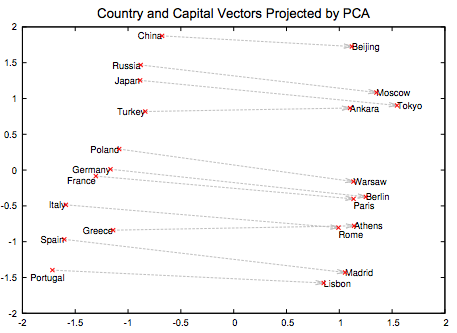
\includegraphics[scale=0.5]{compositionality.png}
	\caption{Compositionality in Word Vectors}
	\label{fig1}
\end{figure}

 \section{Approaches}

\subsection{Word vectors using distributional representations}
Our first approach the problem of Twitter paraphrase detection was to train word vectors with Wordvec, Google's implementation of the Skip-gram algorithm developed by Mikilov et al in Google \cite{Mikolov}, and assign a similarity score between two tweets that is an aggregate of the similarities between individual words in the tweets.  More precisely, we define the distance metric $D_{tweets}$ for two tweets $t_1$ and $t_2$, as the following:

$$D_{tweets}(t_1, t_2) = \sum_{w_i \in t_1} \sum_{w_j \in t_1} D_{cosine}(vec(w_i), vec(w_j))$$\\

where

$$D_{cosine}(x, y) = \frac{x^Ty}{\left \| x \right \| \left \|y \right \|}$$

and $vec(x)$ is the vector representation of word $x$, as learned by the Skip Gram model, which one will detail in the next paragraph.  A pair of tweets is then predicted to be a paraphrase if this distance is above a certain threshold.  We learn this threshold using grid search, which is an exhaustive search over all values applicable to a variable with a constrained range.\\
\indent The idea behind Skip-gram is to learn word vector representations that are good at predicting nearby words.  Skip-gram furthermore models each word as having both an 'input' and an 'output' form, which reflects the directional relation between word pairs.  Specifically: given a sequence of training words $w_1, W_2, w_3 .... w_T$, the objective of the Skip-Gram model is to minimize the average log probability:

$$\frac{1}{T} \sum_{t=1}^T \sum_{-c \leq j \leq c, j \neq 0} logp(w_{t+j}|w_t)$$

where $c$ is the training context, which gives the size of the neighborhod of of $w_t$ to look at, and which may depend on $w_t$. The size of $c$ can be tuned to trade off accuracy (a higher $c$ value) with efficiency (lower $c$). Specifically, Skip Gram defines $p(w_{t+j}|w_t)$ using the softmax function:

$$p(w_O|w_I) = \frac{exp(v_{wo}'^Tv_{wI})}{\sum_{w=1}^W exp(v_w^Tv_{wI})}$$

Where $v_w$ and $v_w'$ are 'input' and 'output' representations of $w$ and $W$ is the number of words in the vocabulary.  This expression, however, is in general computationally infeasible; as an alternative, in practice, Mikilov et al use Hierarchical softmax as an approximation of the softmax function, which defines the probability of one node given abnother by a random walk down a binary tree of the output layer with the  $W$ words as the leaves, and represents the probability of child nodes explicitly for each word.  The math will be excluded here for the sake of brevity. \\
\indent Using this model on words alone, we get the undesireably low accuracy of 64\%, which does not compare well to the baseline of 72\%.  We therefore extend this model by learning vectors for bigrams and trigrams as well, and including phrase vector averaging.  What this means is that we represent each sentence (tweet) not only as a vector over word vectors, but also over word vector objects that correspond to the bi- and trigrams in the sentence.  The modified similarity function then becomes the following:\\

$$D_{tweets}'(t_1, t_2) = \sum_{n=1}^{n=3} \sum_{
\substack{\phi_i \in t_1 \\  |\phi_i| = n}} 
\sum_{\substack{\phi_j \in t_1 \\  |\phi_j| = n}} 
D_{cosine}(vec(\phi_i), vec(\phi_j))$$

Where $\phi_i$ of length $n$ is an $n$-gram in a tweet

\subsubsection{Example}
Consider the input $D$, where $D_T$ is a corpus containing $T$ words, $w_1, W_2, w_3 .... w_T$. For concreteness we can say that D is a corpus of $N$ tweets sampled from Twitter in May 2013.  We now break each tweet into a vector of its words and its bigrams and trigrams (which we term 'phrases'), each of which will be assigned a numerical vector representation, which we will now calculate.  We begin with a random initialization over the vector for each word/phrase, the dimensionality of which we determine based off of empirical results. Then, until we have reached convergence, we compute the gradient of the log likelihood (defined above), parametrized by Hierarchical softmax, and update our word vectors. When convergence comes, we have a word vector representation for each word and each phrase.  
Using these dense vector representations, we can now compare tweets.  We iterate over all pairs of phrases between the two tweets, and take the cosine difference between those phrases.  The similarity score of the two tweets is now the average of these distances of pairs.  If the similarity score is high, we say that they are paraphrases; if it is low we say that they are not.\\
\indent Each tweet can furthermore be assigned a vector representation itself, by aggregating its word vectors in a hierarchical way.  There is an intuitive interpretation that we can now glean from these aggregate vectors.  By observing which words have high values for different elements in the vector, we can determine the semantic meaning of each dimension in the vector. For instance, one might find that all tweets $w_k$ dealing with sports have a high value for $w_{k5}$, whereas tweets about social rights have a high $w_{k18}$. This would indicate that the fifth dimension of the word-vector space corresponded to the general semantic topic of sports, and the 18th to issues of social justice.\\

\subsection{Dynamic Pooling and Unfolding Recursive Autoencoders for Paraphrase Detection}
In this section, we describe a state-of-the-art work \cite{richard} on using dynamic pooling and unfolding recursive autoencoders (RAE) for paraphrase detection.\\
\subsubsection{Model}
The model used here are Neural networks. Neural networks are especially useful in automatically learning features from data. This is much more powerful than manually specifying features to the classifier. A very powerful idea called neural language models was first introduced by Bengio et al. \cite{bengio}. The idea is to jointly learn an embedding of words into an $n$-dimensional vector space and these vectors can be used to predict how likely a word is given its context. A word embedding matrix $L \in \mathbf{R}^{n \times |V|}$, where $|V|$ is the size of the vocabulary is obtained by running gradient descent on the network. Once this training is done we can obtain a word's vector as just a column in $L$.\\
The goal of autoencoders is to learn a representation of their inputs. In this experiment we used recursive autoencoders to learn representations for sentences. The autoencoder uses a neural network layer to compute the parent representation. We then decode the vectors of the children in a reconstruction layer and compute the Euclidean distance between the two as the reconstruction error. For each of the children, we recursively compute the reconstruction loss for their children as well. The goal of the training is to minimize the reconstruction error across all inputs pairs. 
\subsubsection{Algorithm}
For a given sentence, a parse tree is obtained initially. A binary parse tree for a sentence is of the form of triplets of the parents with children: $(p \rightarrow c_1c_2)$. Each child can either be an input word vector $x_i$ or a nonterminal node in the tree. We now can compute parent representations using its two children $(c_1, c_2)$ using a neural network layer:\\
\begin{equation}
p = f(W_e[c_1;c_2] + b)
\end{equation}
where $[c1;c2]$ is the concatenation of the two children, $f$ is an tanh activation function and $W_e \in \mathbf{R}^{n \times 2n}$ the encoding matrix that we want to learn.\\
To assess these $n$-dimensional representation of a parent $p$ we decode the vectors of its direct children into a reconstruction layer and compute the Euclidean distance between the original input and its reconstruction:\\
\begin{equation}
[c^\prime_1;c^\prime_2] = f(W_dp + b_d)
\end{equation}
\begin{equation}
E_{rec}(p) = ||[c_1;c_2] - [c^\prime_1;c^\prime_2]||^2
\end{equation}
The training objective is the minimization of all reconstruction error of the input pairs at nonterminal nodes $p$ in a given parse tree T:\\
\begin{equation}
E_{rec}(T) = \sum_{p \in T} E_{rec}(p)
\end{equation}\\
The unfolding recursive autoencoder is the same as the standard RAE with the only difference being that a reconstruction is created for the entire spanned subtree under each node. The reconstruction error is now computed as a concatenation of all the leaf nodes beneath a non-terminal node.\\
We now use a dynamic pooling pooling method to convert a similarity matrix $S$ generated by sentences of lengths $m$ and $n$ to a matrix $S_{pooled}$ of fixed length $n_p \times n_p$. The idea is to partition the rows and columns in $S$ into $n_p$ roughly equal parts. $S_{pooled}$ is defined as the matrix of the minimum values of each rectangular region within this grid.\\
Finally, a classifier is trained on this matrix which takes as input a matrix and returns a binary decision of whether the two sentences are paraphrases or not.\\
\subsubsection{Example}
Given two sentences and their parse trees $T_1$ and $T_2$, the unfolding recursive neural network will first compute features for these two sentences using the algorithm described above. We then compute the euclidean distance between all word and phrase vectors of the two sentences. This will form the $S$ matrix. We then compute the $S_{pooled}$ matrix as stated above. When this is given to the classifier, it will make a decision of whether the sentences are paraphrases or not.\\

\subsection{GloVe distributed representations}
A recent exciting development in the class of algorithms using dense word vector representations is GloVe, developed at Stanford by Pennington, Socher and Manning. It addresses the problem that standard co-occurrence models are succeptable to noise: The vast majority of co-occurrences in the matrix $X$ will tend to be ones that happen very rarely, and without much particular semantic significance. Even just the 0 entries of $X$ will tend to account for 75-95\% of data. Furthermore, some words that co-occur extremely commonly have little semantic relevance, such as "the" along with any noun. To compensate for this, Pennington et al introduce a weighting function into the least-squares error which lowers the impact of common co-occurrences as well as the least common ones. Furthermore, by ensuring that the function approaches 0 as co-occurrence approaches 0, one naturally excludes all pairs which do not co-occur in the corpus from the calculations, which seems intuitively to make sense, and has the benefit of speeding up calculation significantly. Pennington et al demonstrate that, as a result of using only nonzero co-occurrence values, these methods run in approximately $O(|C|^{0.8})$ , where $|C|$ is the size of the corpus. The objective they propose furthermore claims to address several problems with loss functions of other unsupervised methods based on co-occurrence, such as skip-gram and ivLBL. \cite{GloVe}\\

\subsection{Classifier with word vector features and other features}
Building off the previously described methods, we construct a SVM classifier using features derived from word vectors as features, in addition to other more standard NLP features.  The features we used in total are the following, for a pair of tweets $(t_1, t_2)$:

\begin{enumerate}
\item L1 similarity between $t_1$ and $t_2$ (from word vectors)
\item Cosine similarity between $t_1$ and $t_2$ (from word vectors)
\item Count of matching NER tags
\item 1-gram (word) overlap
\item 2-gram overlap
\item 3-gram overlap
\end{enumerate}

In order to calculate the first two features, we use any of the above-described methods to calculate word- and phrase vectors associated with a tweet. We then average these vectors to make a single vector to represent the tweet as a whole.  As previously mentioned, this technique makes semantic sense, as addition of word vectors simulates composition of their meaning; this final vector is thus a reasonable representation for the meaning of the tweet as a whole.  Once we have a single vector representation for each tweet, we can apply standard distance metrics to the pair, resulting in features 1 and 2 above.\\
\indent To obtain the third feature, we use the Stanford NER (named entity recognition) tagger to assign NER tags to words in each tweet, and then simply count how many tags are shared between the two.  This is a simple and effective way to get an idea of if they are discussing the same topic, which is naturally important in paraphrase detection.  Note however that this alone is not sufficient to determine paraphrase: the tweets ``I never appreciated the connection between \#affinefunctions and \#triangleinequality before I knew the grt. and benfcnt. Earl Goldberg, \#224M" and ``dayum Adam G so tall and hand-some" may both be correctly identified as referring to the entity ``Adam Goldberg", but are about different topics and shouldn't be classified as paraphrases.\\
\indent The final three features are counts of exact n-gram overlap.  This is more or less as it sounds.  The 2-gram overlap of two tweets, for instance, is a count of how many pairs of consecutive words they share.  These features help capture similarity in topic, as with the NER features, and furthermore help capture the interaction between topics, which is what tripped us up in the last example (where the topic ``Adam Goldberg" was shared between the two tweets, but was interacting with different topics himself.) \\
\indent We run this classifier with both the linear and RBF (radial basis function) kernel.  The difference between these two is not easy to explain intuitively, and not worth explaining mathematically for the purposes of this paper; but it may help to think of the RBF kernel as a low band pass filter, a technique which is also used for instance in image processing to smooth images. \cite{RBF}  We furthermore use simple logistic regression, which is labeled as 'LinearFactory' in the plots.

\begin{center}
\begin{tabular}{| c | c | c | c |}
\hline
 Method & Precision & Recall & F1 \\ \hline
test1 & 0.501 & 0.547 & 0.326 \\ \hline
 test2 & 0.726 & 0.751 & 0.74 \\ 
 \hline
\end{tabular}
\end{center}

\section{Results}
TODO melvin write here

\begin{figure}
	\centering
	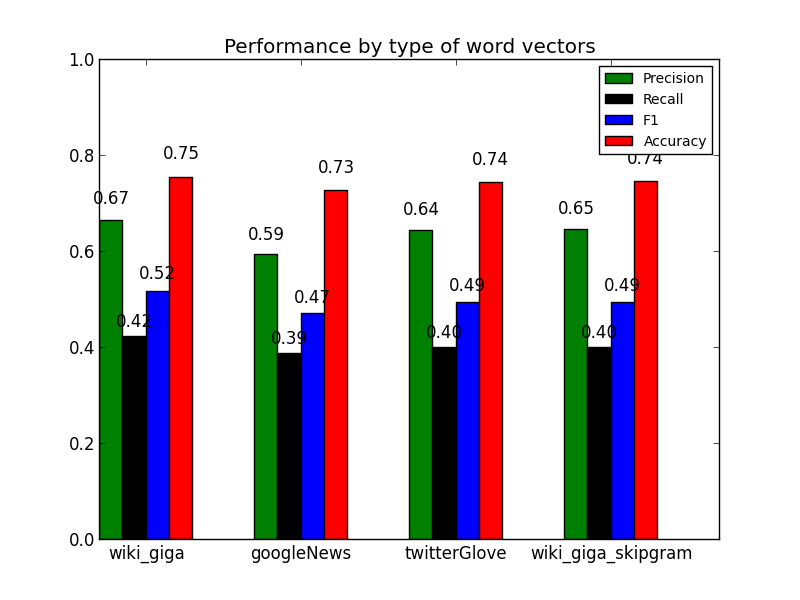
\includegraphics[scale=0.4]{cmp_vecs.png}
	\caption{Performance on Different word vectors}
	\label{vectorSelect}
\end{figure}

\begin{figure}
	\centering
	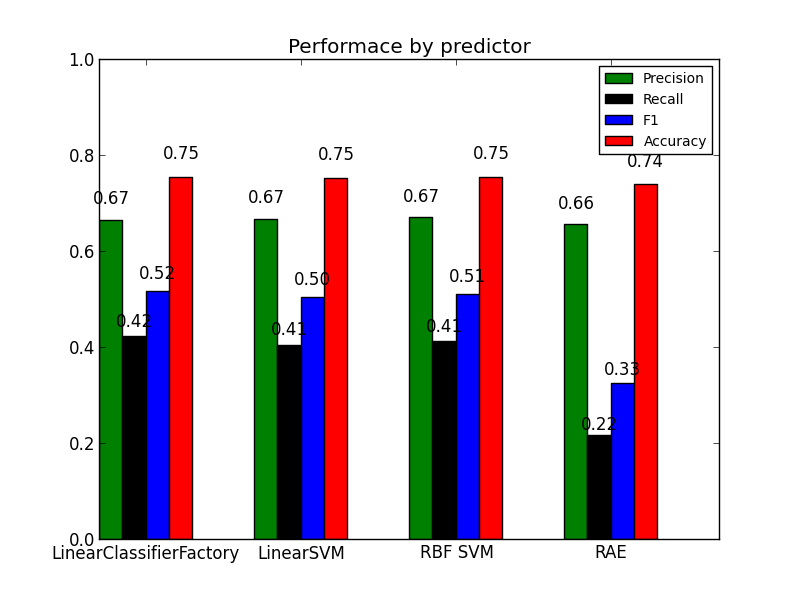
\includegraphics[scale=0.4]{cmp_predictors.png}
	\caption{Performance for different predictors}
	\label{predSelect}
\end{figure}

\section{Error Analysis}
TODO(Melvin) - write me


\begin{figure}
	\centering
	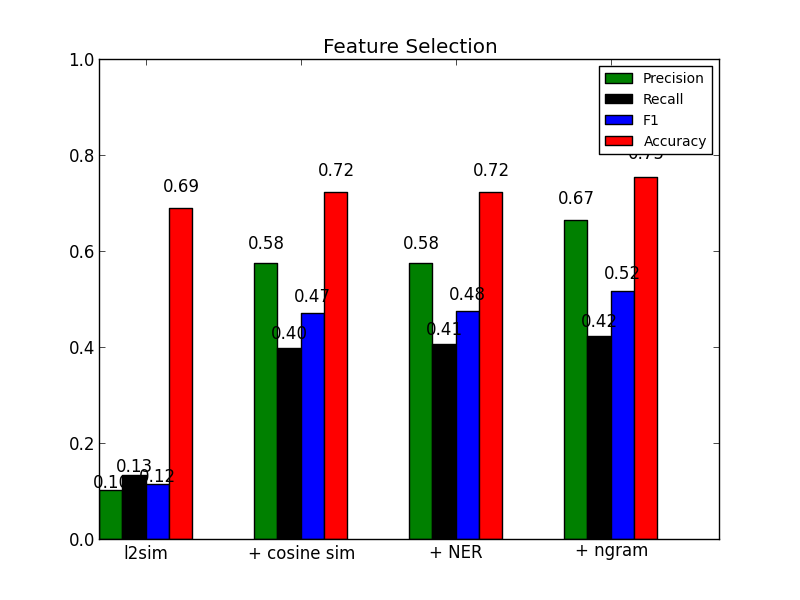
\includegraphics[scale=0.4]{ft_select.png}
	\caption{Forward feature selection}
	\label{feat}
\end{figure}


\section{Conclusion}
TODO(melvin) - write me

\section{Future Work}
TODO melvin
There are several things we can do to improve the accuracy of our current model.  Following is a list of the next things we will work on




% trigger a \newpage just before the given reference
% number - used to balance the columns on the last page
% adjust value as needed - may need to be readjusted if
% the document is modified later
%\IEEEtriggeratref{8}
% The "triggered" command can be changed if desired:
%\IEEEtriggercmd{\enlargethispage{-5in}}

% references section

% can use a bibliography generated by BibTeX as a .bbl file
% BibTeX documentation can be easily obtained at:
% http://www.ctan.org/tex-archive/biblio/bibtex/contrib/doc/
% The IEEEtran BibTeX style support page is at:
% http://www.michaelshell.org/tex/ieeetran/bibtex/
%\bibliographystyle{IEEEtran}
% argument is your BibTeX string definitions and bibliography database(s)
%\bibliography{IEEEabrv,../bib/paper}
%
% <OR> manually copy in the resultant .bbl file
% set second argument of \begin to the number of references
% (used to reserve space for the reference number labels box)
\begin{thebibliography}{1}

\bibitem{derczynski}
Leon Derczynski, Allan Ritter, Sam Clark, Kalina Bontcheva, 
Twitter Part-of-Speech Tagging for All: Overcoming Sparse and Noisy Data.
RANLP 2013.

\bibitem{OConnor}
Brendan O’Connor, Michel Krieger, David Ahn,
Tweetmotif: Exploratory Search and Topic Summarization for Twitter.
ICWSM 2010.

\bibitem{zane}
Wei Xu, Alan Ritter, Chris Callison-Burch, William B. Dolan, Yangfeng Ji, 
Extracting Lexically Divergent Paraphrase from Twitter. 
2014 Association for Computational Linguistics.

\bibitem{richard}
Richard Socher, Eric H. Huang, Jeffrey Pennington
, Andrew Y. Ng, Christopher D. Manning, Dynamic Pooling and Unfolding Recursive
Autoencoders for Paraphrase Detection, NIPS 2011.

\bibitem{Mikolov}
Tomas Mikolov, Ilya Sutskever, Kai Chen,
Greg Corrado, Jeffry Dean
Distributed Representations of Words and Phrases
and their Compositionality, 2013

\bibitem{GloVe}
Jeffrey Pennington, Richard Socher, Christopher D. Manning
GloVe: Global Vectors for Word Representation

\bibitem{Wordvec}
Richard Socher and Christopher Manning
Deep	 Learning for NLP
NAACL 2013, Atlanta

\bibitem{RBF}
Alex J. Smola, Bernhard Sch{\"o}lkopf, Klaus-Robert M{\"u}ller
The connection between regularization operators and support vector kernels
 22 December 1997

\bibitem{Gigaword}
English Gigaword Fifth Edition
Online Dataset description
https://catalog.ldc.upenn.edu/LDC2011T07

\bibitem{Das}
Dipanjan Das and Noah A. Smith
Paraphrase Identification as Probabilistic Quasi-Synchronous Recognition
2009 ACL and AFNLP

\end{thebibliography}




% that's all folks
\end{document}


